A \emph{Relation} defines the relationship between two Objects. Every Object can have zero or more \emph{Relations}.
\par
An example of a \emph{Relation} is the relation between \emph{Project} and \emph{Tasks}. One \emph{Project} can have zero or more \emph{Tasks}. One \emph{Tasks} must have a \emph{Project}.

\begin{figure}[ht]
	\begin{center}
		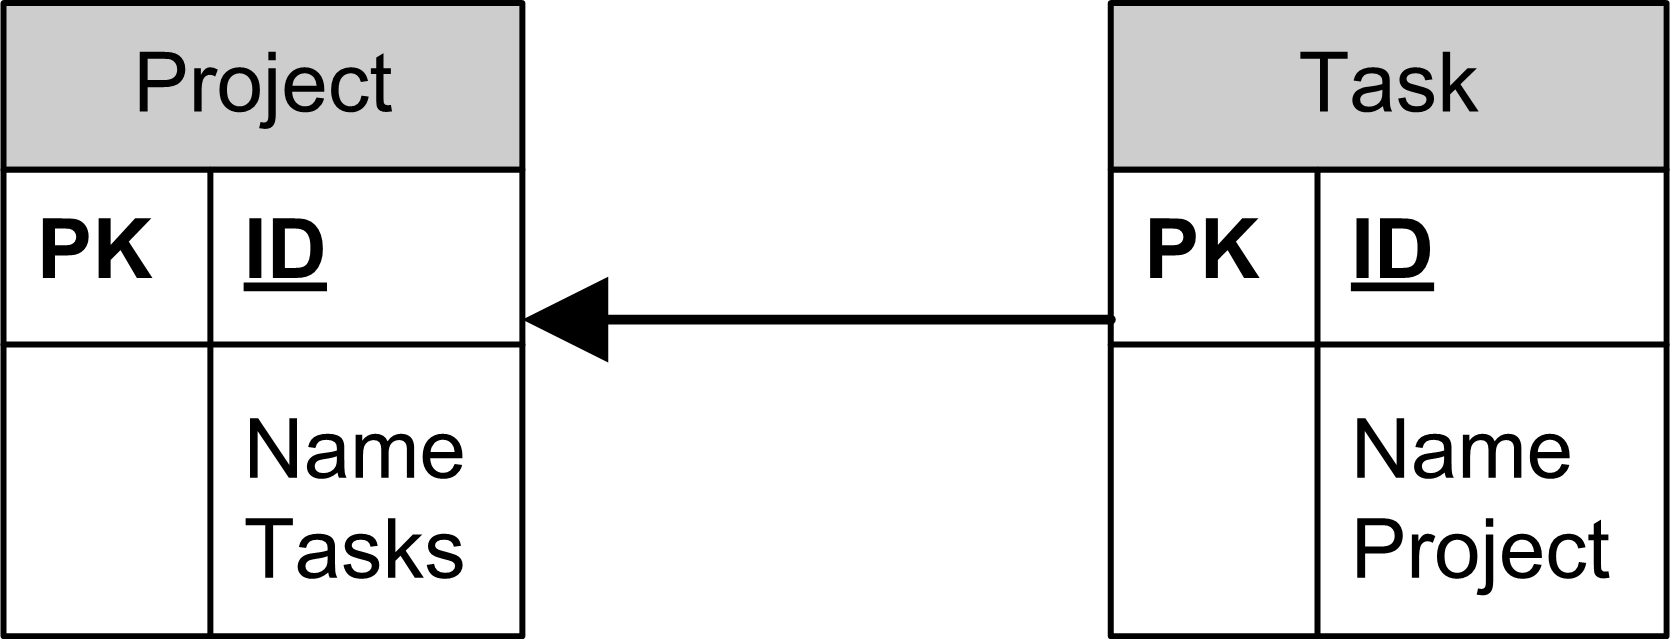
\includegraphics[width=0.6\textwidth]{images/Rel_1_n_Project_Tasks.png}
		\caption{Example for a \emph{Relation}}
		\label{example_for_relation}
	\end{center}
\end{figure}


% ----------------------------------------------------------------- Modeling relation -----------------------------------------------------------------
\subsubsection{Modeling a relation}
A Relation can be defined by creating an object of type \emph{Relation} and two \emph{RelationEnd} objects. This can be done by
\begin{itemize}
	\item creating an Relation Object. 
	\item invoking the \emph{Create Relation} method on an \emph{ObjectClass} instance.
\end{itemize}

\emph{RelationEnd} objects will be created automatically.

\par
Relations are edited in the \emph{Relation Editor}. The \emph{Relation Editor} is a custom \emph{FullObjectView} created by us.

\begin{figure}[ht]
	\begin{center}
		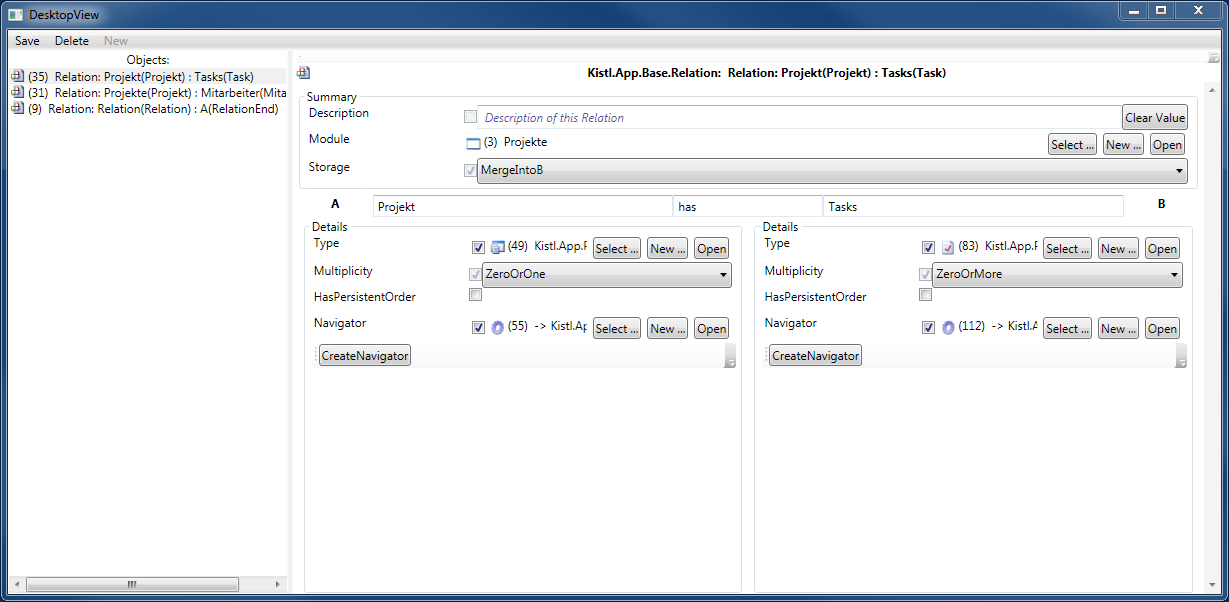
\includegraphics[width=0.9\textwidth]{images/ScreenShot_Rel_Project_Task.png}
		\caption{Example for editing a \emph{Relation}}
		\label{example_for_editing_relation}
	\end{center}
\end{figure}

% ----------------------------------------------------------------- Attributes of a relation -----------------------------------------------------------------
\subsubsection{Attributes of a relation}

\begin{figure}[ht]
	\begin{center}
		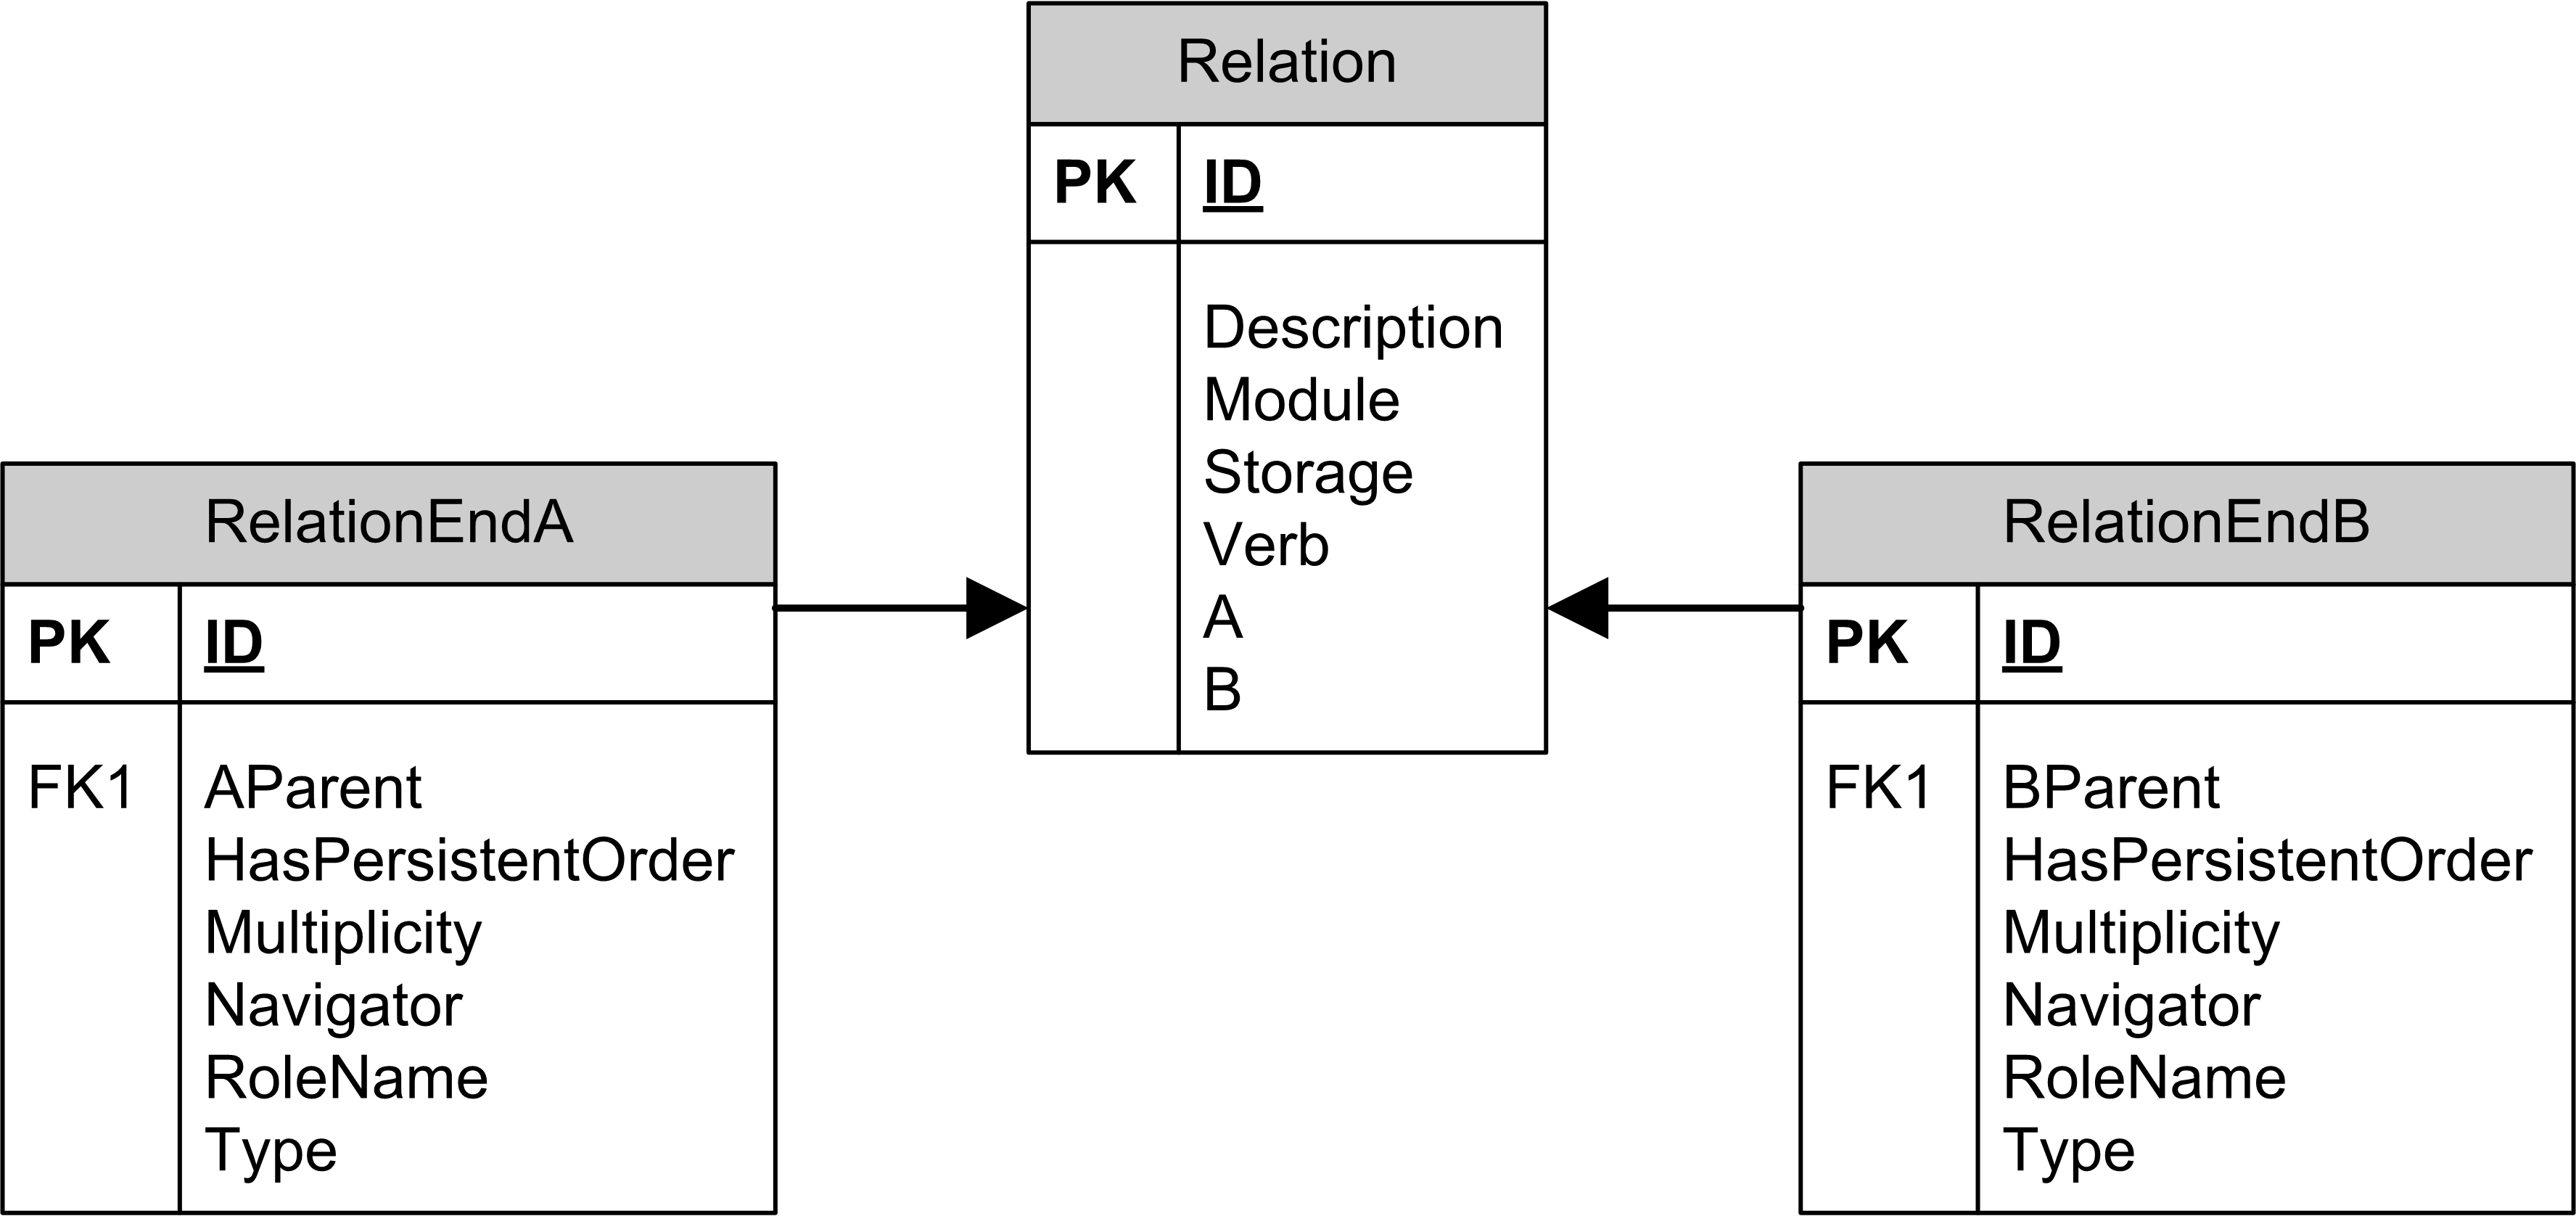
\includegraphics[width=0.9\textwidth]{images/Rel_Attributes.png}
		\caption{Attributes of a relation}
		\label{attributes_of_a_relation}
	\end{center}
\end{figure}

A \emph{Relation} has these attributes:
\begin{descriptionBorder}
	\item[Description] 	{ A text property used to describe the current relation }
	\item[Module] 		{ The \emph{Module} which is introducing the current relation }
	\item[Storage] 		{ The \emph{StorageType} of the current relation }
	\item[Verb] 		{ 	A verb used to name the current relation. 
							The verb is used in conjunction with the role names of the \emph{RelationEnd} objects to model a unique relation name. 
							This relation name will be used e.g. for the database FK Contraint name.}
	\item[A] 			{ The \emph{RelationEnd} A of the current relation }
	\item[B] 			{ The \emph{RelationEnd} B of the current relation }
\end{descriptionBorder}

A \emph{RelationEnd} has these attributes:
\begin{descriptionBorder}
	\item[AParent] { \emph{Relation} object if this \emph{RelationEnd} is the A-Side of the current relation. Otherwise \emph{NULL} }
	\item[BParent] { \emph{Relation} object if this \emph{RelationEnd} is the B-Side of the current relation. Otherwise \emph{NULL} }
	\item[HasPersistentOrder] { Specifies that the list is ordered. Applies only to lists  }
	\item[Multiplicity] { The \emph{Multiplicity} of the current \emph{RelationEnd} }
	\item[Navigator] { An optional \emph{Navigator} }
	\item[RoleName] { Name of the role of the current \emph{RelationEnd} }
	\item[Type] { \emph{ObjectClass} to which the current \emph{RelationEnd} points }
\end{descriptionBorder}

There are four \emph{StorageTypes} defined:
\begin{descriptionBorder}
	\item[MergeIntoA] { The relation information is stored with the A-side database table }
	\item[MergeIntoB] { The relation information is stored with the B-side database table }
	\item[Replicate] { The relation information is stored on both sides of the relations database tables }
	\item[Separate] { The relation information is stored in a separate database table }
\end{descriptionBorder}

There are three \emph{Multiplicities} defined:
\begin{descriptionBorder}
	\item[ZeroOrOne] { Optional Element (zero or one) }
	\item[One] { Required Element (exactly one) }
	\item[ZeroOrMore] { Optional List Element (zero or more) }
\end{descriptionBorder}

% ----------------------------------------------------------------- 1:n Relation -----------------------------------------------------------------
\subsubsection{1:n Relation}
A \emph{Project} can have zero or more \emph{Tasks}. A \emph{Task} may have one \emph{Project}.

\begin{figure}[ht]
	\begin{center}
		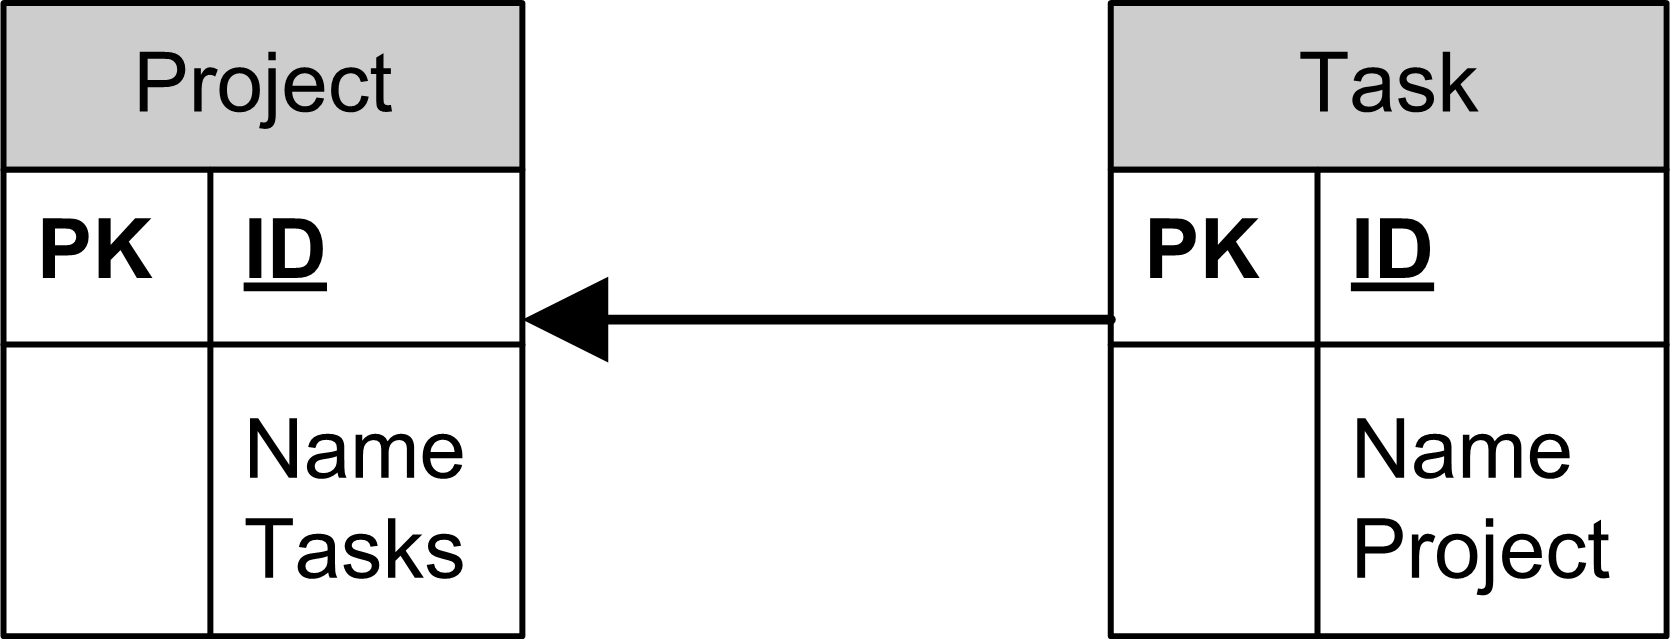
\includegraphics[width=0.6\textwidth]{images/Rel_1_n_Project_Tasks.png}
		\caption{Project/Tasks relation}
		\label{project_tasks_relation}
	\end{center}
\end{figure}

The \emph{Relation} object would be:
\begin{descriptionBorder}
	\item[Storage] 		{ = MergeIntoB }
	\item[Verb] 		{ = has }
\end{descriptionBorder}

The \emph{RelationEnd} A object would be:
\begin{descriptionBorder}
	\item[AParent] { = \emph{Relation}  }
	\item[BParent] { = \emph{NULL} }
	\item[HasPersistentOrder] { = false  }
	\item[Multiplicity] { = ZeroOrOne. If a \emph{Task} must have a \emph{Project} then One. }
	\item[Navigator] { = \emph{Navigator} to Tasks. The result would be a collection of \emph{Tasks} (ICollection\textless Task\textgreater) }
	\item[RoleName] { = Project }
	\item[Type] { = \emph{Task} instance of type \emph{ObjectClass} }
\end{descriptionBorder}

The \emph{RelationEnd} B object would be:
\begin{descriptionBorder}
	\item[AParent] { =  \emph{NULL} }
	\item[BParent] { = \emph{Relation} }
	\item[HasPersistentOrder] { = false  }
	\item[Multiplicity] { = ZeroOrMore }
	\item[Navigator] { = \emph{Navigator} to the parent \emph{Project}. The result would be a reference to a \emph{Project}  }
	\item[RoleName] { = Tasks }
	\item[Type] { = \emph{Project} instance of type \emph{ObjectClass} }
\end{descriptionBorder}

\begin{figure}[ht]
	\begin{center}
		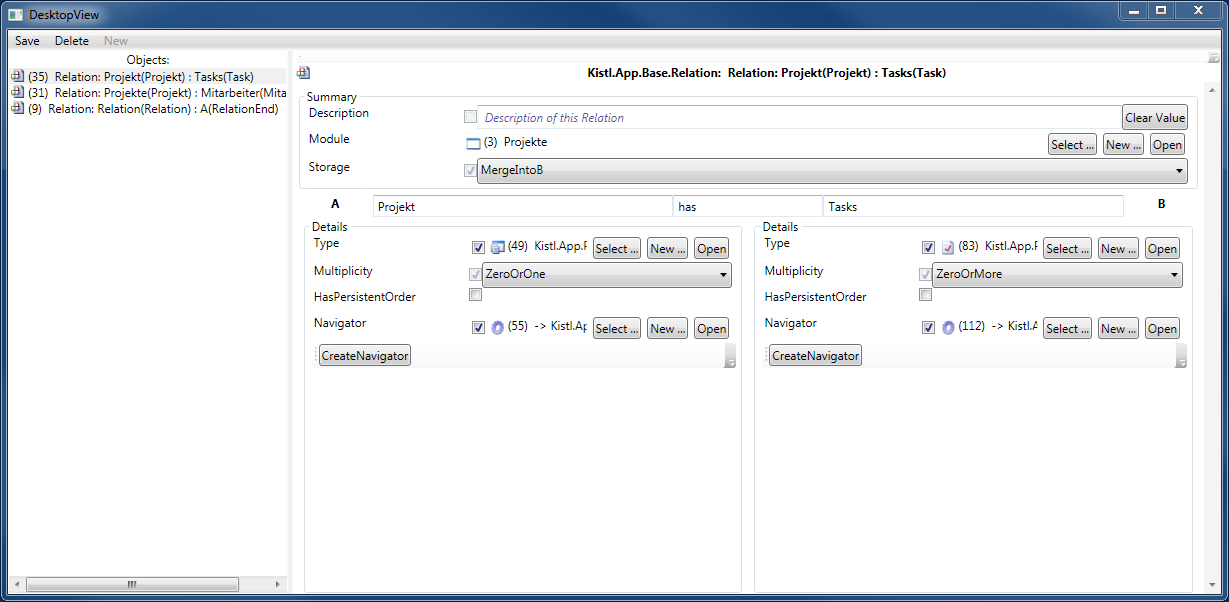
\includegraphics[width=0.9\textwidth]{images/ScreenShot_Rel_Project_Task.png}
		\caption{Editing the \emph{Project}/\emph{Tasks} relation}
		\label{editing_project_tasks_relation}
	\end{center}
\end{figure}

% ----------------------------------------------------------------- n:m Relation -----------------------------------------------------------------
\subsubsection{n:m Relation}
A \emph{Project} can have zero or more \emph{ProjectMembers}. A \emph{ProjectMember} can be assinged to zero or more \emph{Projects}.

\begin{figure}[ht]
	\begin{center}
		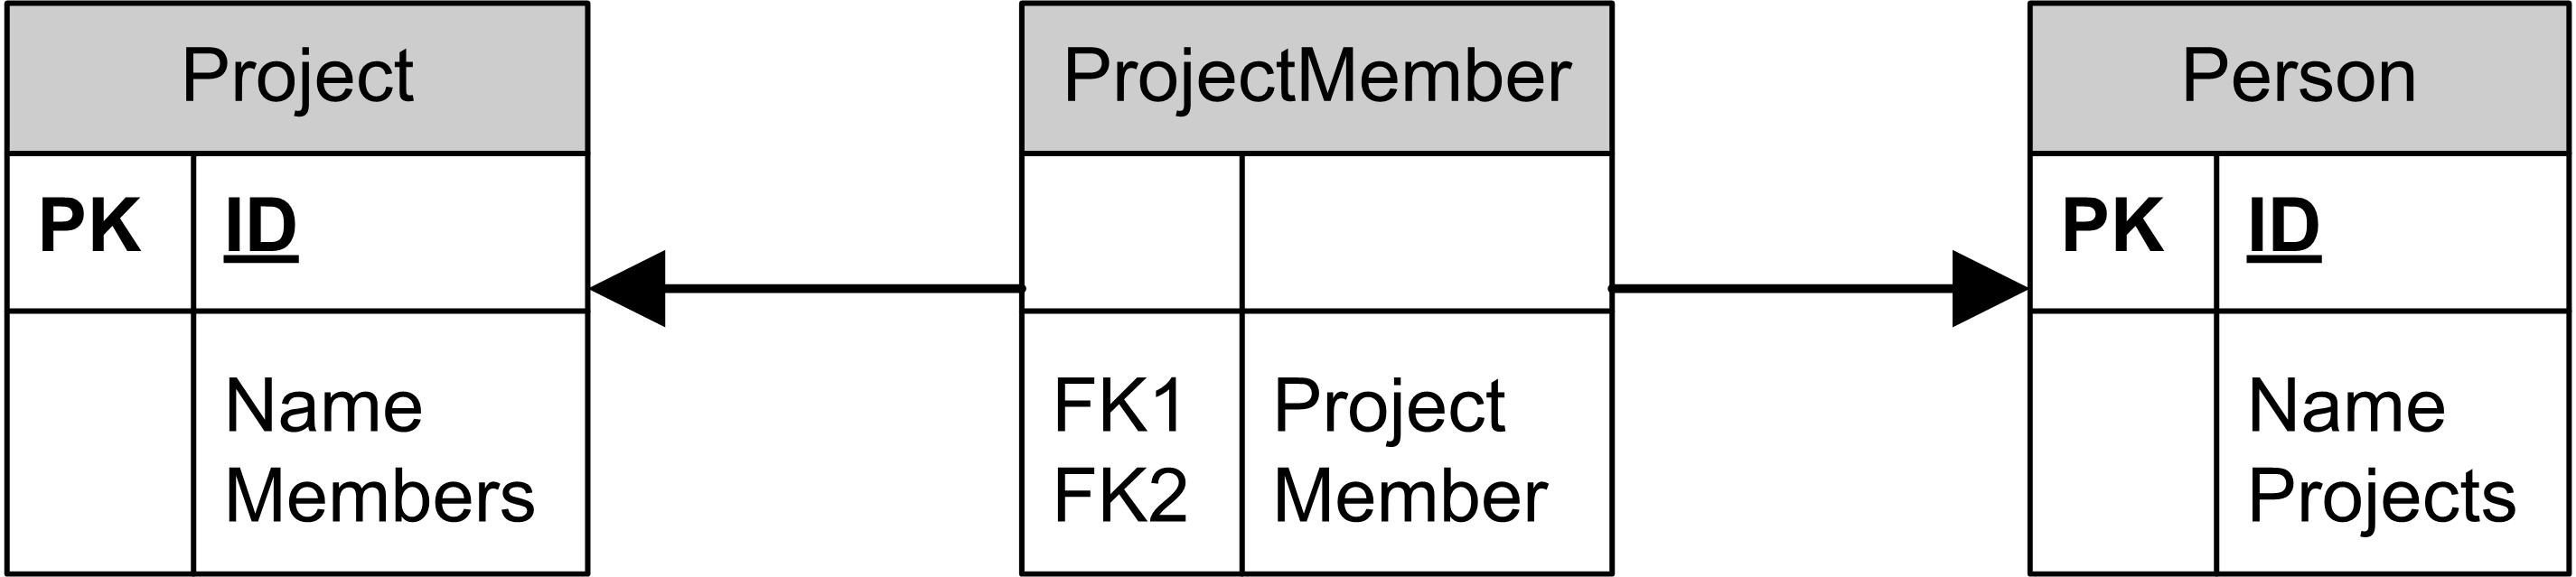
\includegraphics[width=0.6\textwidth]{images/Rel_n_m_Project_Member.png}
		\caption{Project/Member relation}
		\label{project_member_relation}
	\end{center}
\end{figure}

The \emph{Relation} object would be:
\begin{descriptionBorder}
	\item[Storage] 		{ = Seperate }
	\item[Verb] 		{ = has }
\end{descriptionBorder}

The \emph{RelationEnd} A object would be:
\begin{descriptionBorder}
	\item[AParent] { = \emph{Relation}  }
	\item[BParent] { = \emph{NULL} }
	\item[HasPersistentOrder] { = true  }
	\item[Multiplicity] { = ZeroOrMore. }
	\item[Navigator] { = \emph{Navigator} to Persons. The result would be a list of \emph{Persons} (IList\textless Person\textgreater) }
	\item[RoleName] { = Projects }
	\item[Type] { = \emph{Person} instance of type \emph{ObjectClass} }
\end{descriptionBorder}

The \emph{RelationEnd} B object would be:
\begin{descriptionBorder}
	\item[AParent] { =  \emph{NULL} }
	\item[BParent] { = \emph{Relation} }
	\item[HasPersistentOrder] { = true  }
	\item[Multiplicity] { = ZeroOrMore }
	\item[Navigator] { = \emph{Navigator} to the assigned \emph{Projects}. The result would be a list of \emph{Projects} (IList\textless Project\textgreater)  }
	\item[RoleName] { = Member }
	\item[Type] { = \emph{Project} instance of type \emph{ObjectClass} }
\end{descriptionBorder}

\begin{figure}[ht]
	\begin{center}
		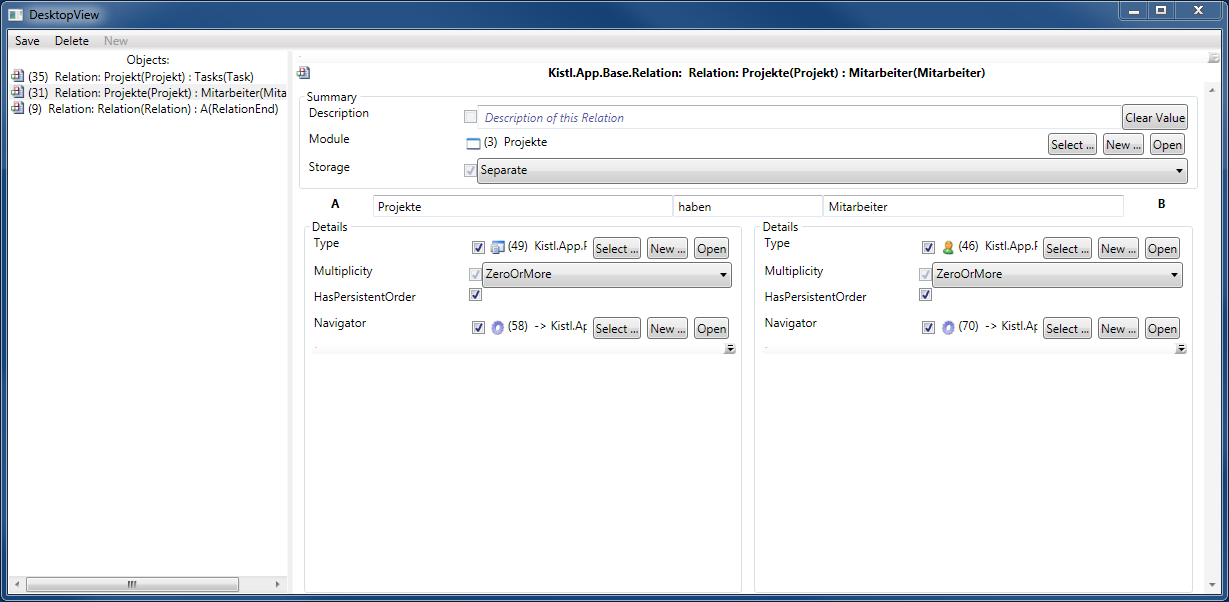
\includegraphics[width=0.9\textwidth]{images/ScreenShot_Rel_Project_ProjectMember.png}
		\caption{Editing the \emph{Project}/\emph{Member} relation}
		\label{editing_project_member_relation}
	\end{center}
\end{figure}

% ----------------------------------------------------------------- 1:1 Relation -----------------------------------------------------------------
\subsubsection{1:1 Relation}
A \emph{Relation} must have a \emph{RelationEnd} A. A \emph{RelationEnd} may have a AParent \emph{Relation} if it's a A \emph{ReleationEnd}.

\begin{figure}[ht]
	\begin{center}
		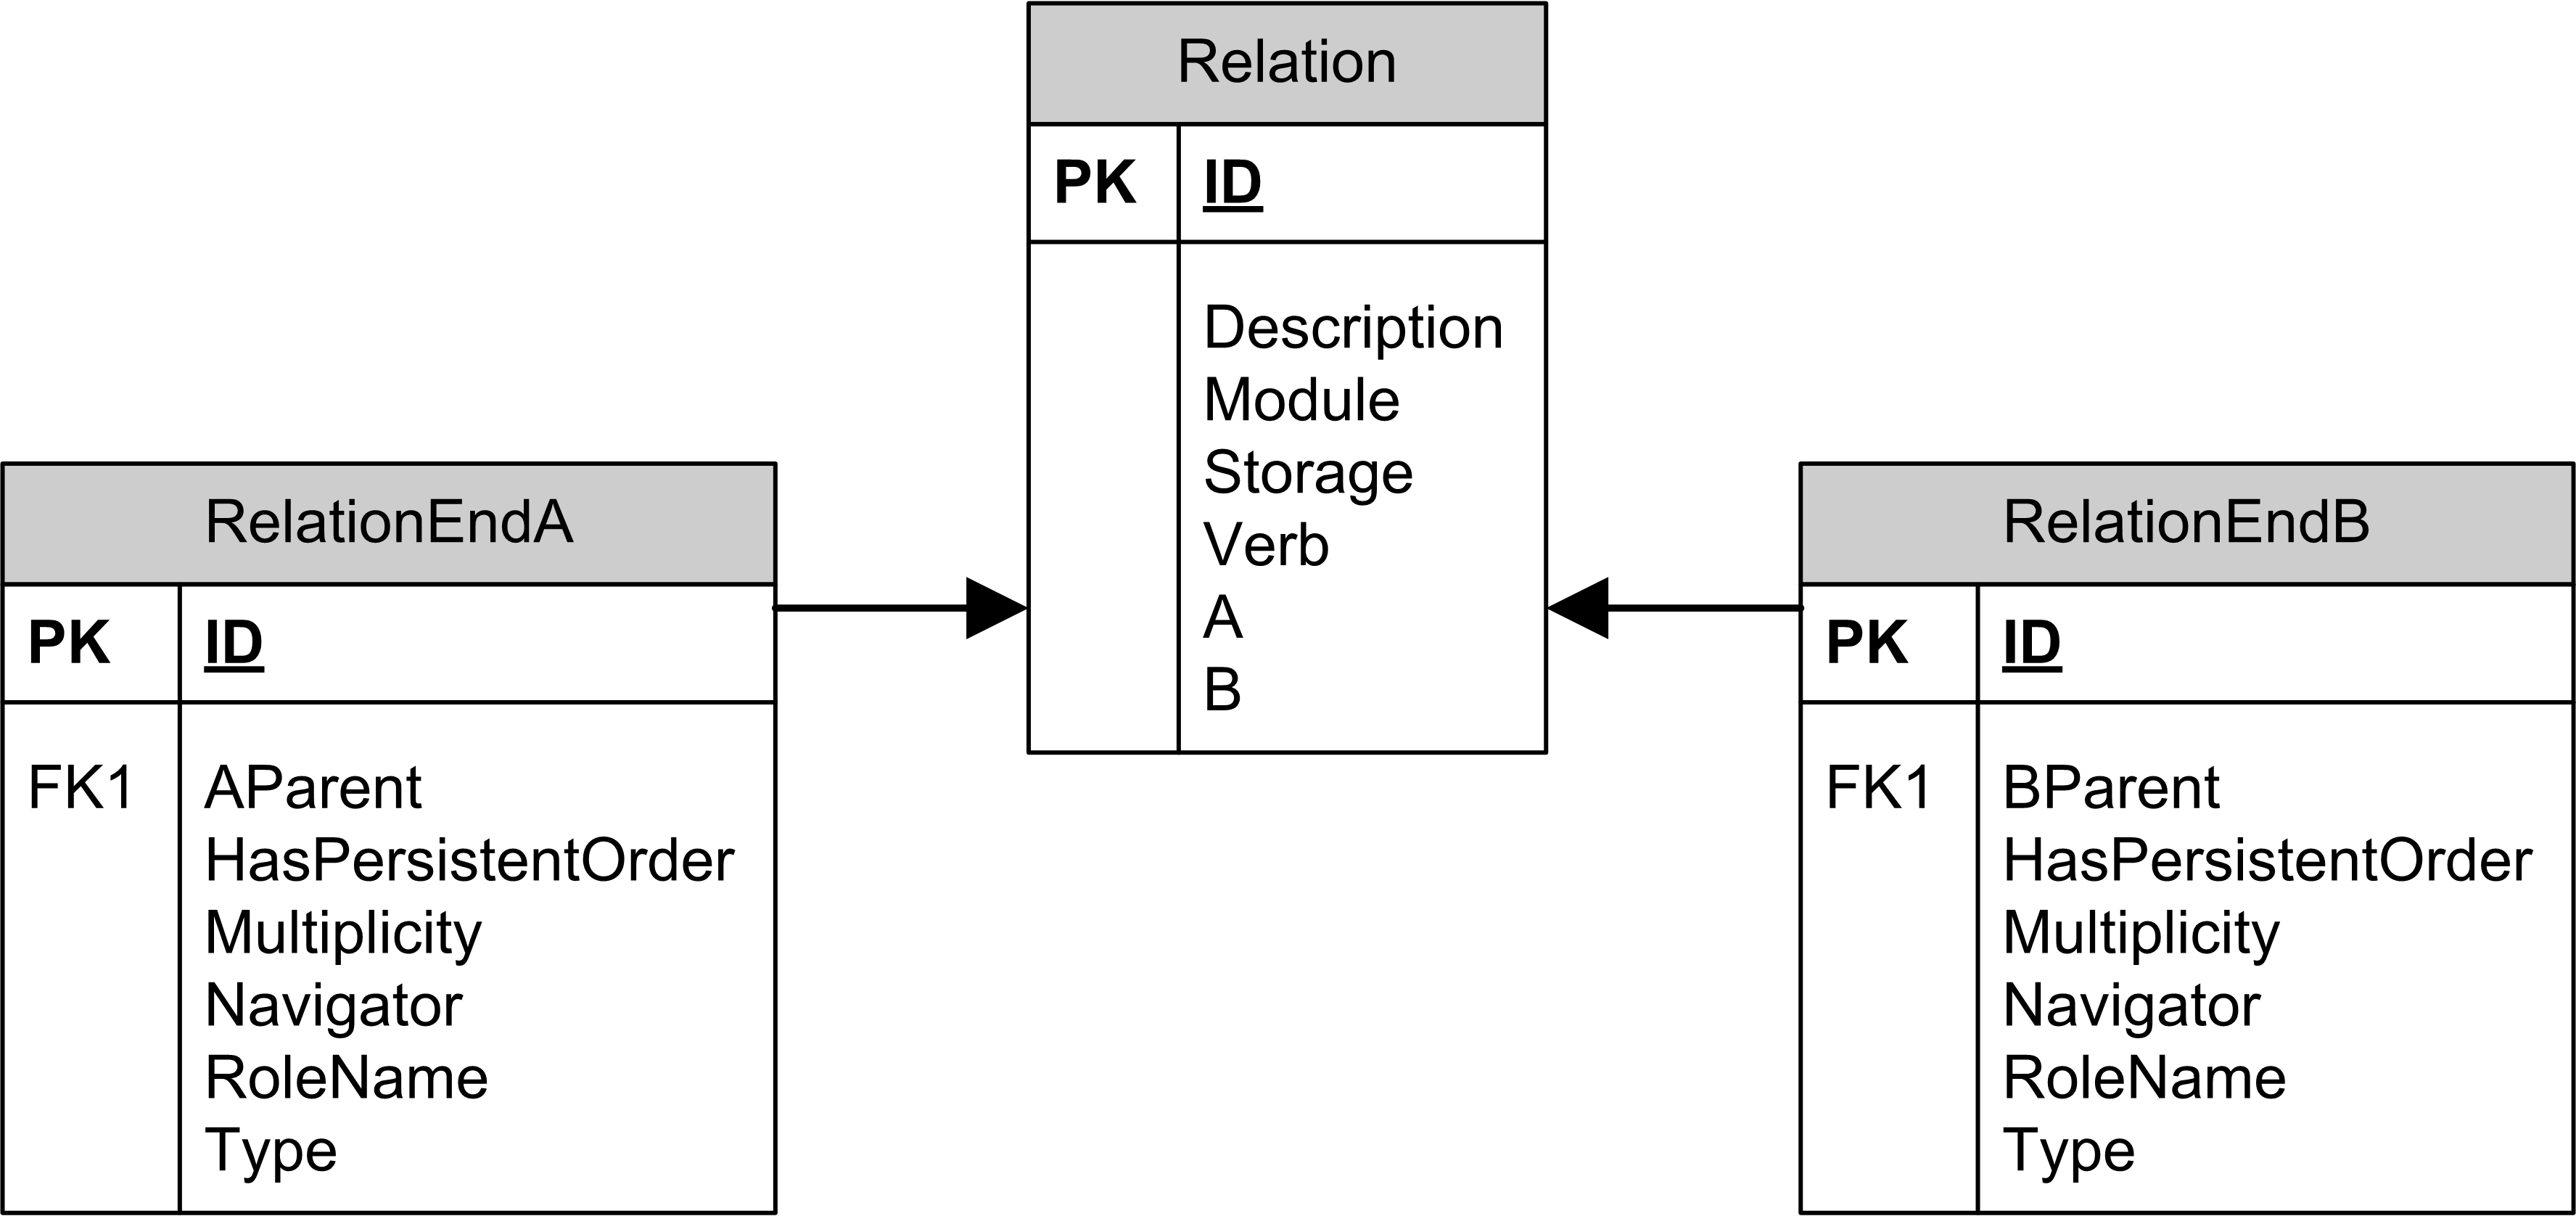
\includegraphics[width=0.9\textwidth]{images/Rel_Attributes.png}
		\caption{Relation/RelationEnd relation}
		\label{relation_relationend_relation}
	\end{center}
\end{figure}

The \emph{Relation} object would be:
\begin{descriptionBorder}
	\item[Storage] 		{ = MergeIntoA }
	\item[Verb] 		{ = hasA }
\end{descriptionBorder}

The \emph{RelationEnd} A object would be:
\begin{descriptionBorder}
	\item[AParent] { = \emph{Relation}  }
	\item[BParent] { = \emph{NULL} }
	\item[HasPersistentOrder] { = false  }
	\item[Multiplicity] { = ZeroOrOne }
	\item[Navigator] { = \emph{Navigator} to \emph{RelationEnd}. The result would be a reference to a \emph{RelationEnd} }
	\item[RoleName] { = Relation }
	\item[Type] { = \emph{RelationEnd} instance of type \emph{ObjectClass} }
\end{descriptionBorder}

The \emph{RelationEnd} B object would be:
\begin{descriptionBorder}
	\item[AParent] { =  \emph{NULL} }
	\item[BParent] { = \emph{Relation} }
	\item[HasPersistentOrder] { = true  }
	\item[Multiplicity] { = One }
	\item[Navigator] { = \emph{Navigator} to the assigned \emph{Relation}. The result would be a reference to a \emph{Relation}  }
	\item[RoleName] { = A }
	\item[Type] { = \emph{Relation} instance of type \emph{ObjectClass} }
\end{descriptionBorder}

\begin{figure}[ht]
	\begin{center}
		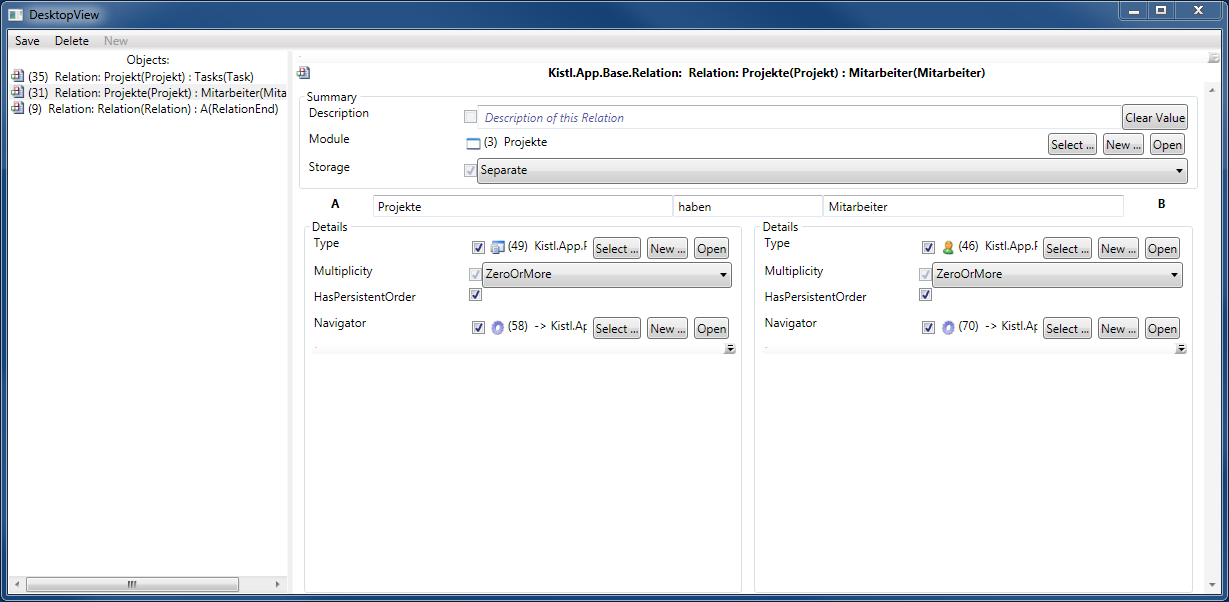
\includegraphics[width=0.9\textwidth]{images/ScreenShot_Rel_Project_ProjectMember.png}
		\caption{Editing the \emph{Relation}/\emph{RelationEnd} relation}
		\label{editing_relation_relationend_relation}
	\end{center}
\end{figure}

% ----------------------------------------------------------------- Multiplicity summary -----------------------------------------------------------------
\subsubsection{Multiplicity and StorageType summary}

\begin{center}
	\begin{tabular}{|p{5cm}|p{5cm}|}
	\hline
		\multicolumn{2}{|c|}{\textbf{1:n}} \\ 
		\multicolumn{2}{|c|}{ Storage = MergeIntoB } \\
	\hline
		\multicolumn{1}{|c|}{\textbf{A}} & \multicolumn{1}{|c|}{\textbf{B}} \\
	\hline
		A.Nav is a collection & B.Nav is nullable \\
		Multiplicity = ZeroOrOne & Multiplicity = ZeroOrMore \\
	\hline
		A.Nav is a collection & B.Nav is not nullable\\
		Multiplicity = One  & Multiplicity = ZeroOrMore \\
	\hline
	\end{tabular}
\end{center}

\begin{center}
	\begin{tabular}{|p{5cm}|p{5cm}|}
	\hline
		\multicolumn{2}{|c|}{\textbf{n:1}} \\ 
		\multicolumn{2}{|c|}{ Storage = MergeIntoA } \\
	\hline
		\multicolumn{1}{|c|}{\textbf{A}} & \multicolumn{1}{|c|}{\textbf{B}} \\
	\hline
		A.Nav is nullable & B.Nav is a collection \\
		Multiplicity = ZeroOrMore & Multiplicity = ZeroOrOne\\
	\hline
		A.Nav is not nullable & B.Nav is a collection \\
		Multiplicity = ZeroOrMore & Multiplicity = One \\
	\hline
	\end{tabular}
\end{center}

\begin{center}
	\begin{tabular}{|p{5cm}|p{5cm}|}
	\hline
		\multicolumn{2}{|c|}{\textbf{n:m}} \\ 
		\multicolumn{2}{|c|}{ Storage = Seperate } \\
	\hline
		\multicolumn{1}{|c|}{\textbf{A}} & \multicolumn{1}{|c|}{\textbf{B}} \\
	\hline
		A.Nav is a collection & B.Nav is a collection \\
		Multiplicity = ZeroOrMore & Multiplicity = ZeroOrMore \\
	\hline
	\end{tabular}
\end{center}

\begin{center}
	\begin{tabular}{|p{5cm}|p{5cm}|}
	\hline
		\multicolumn{2}{|c|}{\textbf{1:1}} \\ 
		\multicolumn{2}{|c|}{ Storage = MergeIntoA } \\
		\multicolumn{2}{|c|}{ Storage = MergeIntoB } \\
		\multicolumn{2}{|c|}{ Storage = Replicate (Not supported yet) } \\
	\hline
		\multicolumn{1}{|c|}{\textbf{A}} & \multicolumn{1}{|c|}{\textbf{B}} \\
	\hline
		A.Nav is nullable & B.Nav is nullable \\
		Multiplicity = ZeroOrOne & Multiplicity = ZeroOrOne \\
	\hline
		A.Nav is nullable & B.Nav is not nullable \\
		Multiplicity = One & Multiplicity = ZeroOrOne \\
	\hline
		A.Nav is not nullable & B.Nav is nullable \\
		Multiplicity = ZeroOrOne & Multiplicity = One \\
	\hline
		A.Nav is not nullable & B.Nav is not nullable \\
		Multiplicity = One & Multiplicity = One \\
	\hline
	\end{tabular}
\end{center}

